\documentclass[11pt,a4paper]{article}
\usepackage[T1]{fontenc}
\usepackage{graphicx}
\usepackage{mathtools}
\usepackage{amssymb}
\usepackage{geometry}
\usepackage{titlesec}
\usepackage{enumitem} % 添加enumitem宏包
\usepackage{amsfonts}
\usepackage{amssymb}
\usepackage{fancyhdr} % 添加fancyhdr宏包 增加页脚
\usepackage{lastpage} % 添加lastpage宏包
\usepackage{graphicx} % 导入graphicx包
\usepackage{gensymb} % 引入gensymb包

\usepackage[UTF8]{ctex}
% 应用fancyhdr宏包的页脚样式
\pagestyle{fancy}
\fancyhf{} % 清除当前的页眉页脚设置
\fancyfoot[L]{免费开源,请勿商用} % 页脚左下方显示文字
\fancyfoot[R]{作者:阿尧} % 页脚右下方显示文字
\renewcommand{\headrulewidth}{0pt} % 去掉页眉的横线
\renewcommand{\footrulewidth}{1pt} % 设置页脚的横线宽度
\usepackage{draftwatermark} %增加水印
\SetWatermarkText{本真题由b站up陈瀚尧探索世界免费开源}
\SetWatermarkScale{0.3} % 可以调整为合适的大小
\SetWatermarkColor{gray!50} % 灰色透明度为50%

% 设置更窄的页面边距
\geometry{left=3cm, right=3cm, top=1cm, bottom=2cm}

% 设置section标题格式
\titleformat{\title}{\bfseries}{\thetitle}{1em}{}

% 设置section之间的距离
\titlespacing*{\section}{0pt}{3.25ex plus 1ex minus .2ex}{1.5ex plus .2ex}

\begin{document}
    \title{中国科学院大学\\2019年招收攻读硕士学位研究生入学统一考试试题\\科目名称:光学}
    \author{制作者:b站up 陈瀚尧探索世界}
    \date{}
    \maketitle
    % 设置section标题不显示序号
    \titleformat{\section}[block]{\normalfont\Large\bfseries}{}{0pt}{}

    % 设置itemize环境的项目符号为空
    \setlist[itemize]{label=} 

    \section{考试须知:}
    \begin{itemize}[topsep=0pt,itemsep=0pt,partopsep=0pt]
        \item 1.本试卷满分为150分,全部考试时间总计180分钟。
        \vspace{-3mm}
        \item 2.所有答案必须写在答题纸上,写在试题纸上或草稿纸上一律无效。
        \vspace{-3mm}
        \item 3.可以使用无字典存储或编程功能的电子计算器。(此条对于25考研可能作废)
    \end{itemize}
    \vspace{-5mm}
    \noindent\rule{\textwidth}{0.5pt} % 添加一条线
    \vspace{-12mm}
    \section*{一、填空题:本题共5小题}
    \begin{enumerate}
        \vspace{0mm}
        \item 发生全反射的条件是\underline{\makebox[2cm]{}}和\underline{\makebox[2cm]{}}
        \vspace{-3mm}
        \item 假定某人在白天的瞳孔直径为2mm。在夜晚的瞳孔直径为4mm,则此人在白天的极限分辨角是\underline{\makebox[2cm]{}},在夜晚的极限分辨角是\underline{\makebox[2cm]{}}。
        \vspace{-3mm}
        \item 焦距为$100mm$放大镜的放大倍率大约是\underline{\makebox[3cm]{}}        
        \vspace{-3mm}
        \item 对于正常人眼,要观察$1m$远的目标,需要调节\underline{\makebox[2cm]{}}视度。个人的远点距离为$-0.5m$,需配的眼镜为\underline{\makebox[2cm]{}}“度”近视镜。
        \vspace{-3mm}
        \item 在一个$3^x$的伽利略望远镜物镜前,加一个焦距为$150mm$的正透镜,则此组合放大镜的视放大率是\underline{\makebox[2cm]{}}倍。
        \vspace{-3mm}
        \item 光学系统的球差是指\underline{\makebox[3cm]{}},轴向色差是指\underline{\makebox[3cm]{}}。
        \vspace{-3mm}
    \end{enumerate}
    \section*{二、画图题:本题共4小题}
    \begin{itemize}
        \item (1) 用作图法求图中垂轴像A'B'对应的物AB
        
        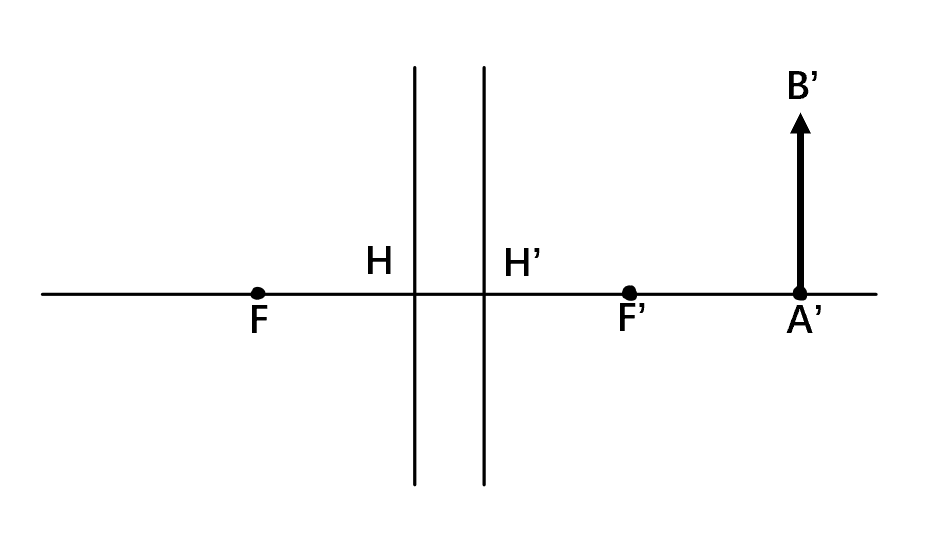
\includegraphics[scale=0.2]{1.png}% 插入图片,按50%的比例缩放
        \vspace{-5mm}
        \item (2) 用作图法求下图薄透镜的焦点F, F'的位置。
         
        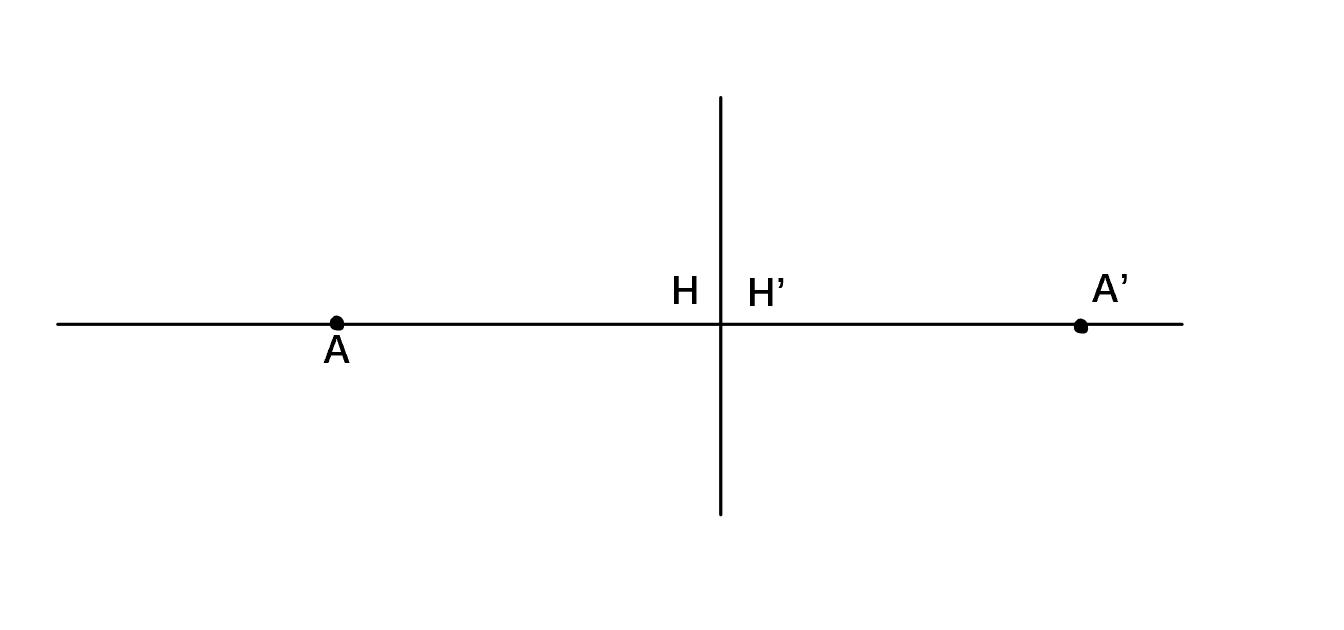
\includegraphics[scale=0.2]{2.png}% 插入图片,按50%的比例缩放
        \vspace{-5mm}
        \item (3) 用作图法求图中垂轴物体AB的像A'B'
        
        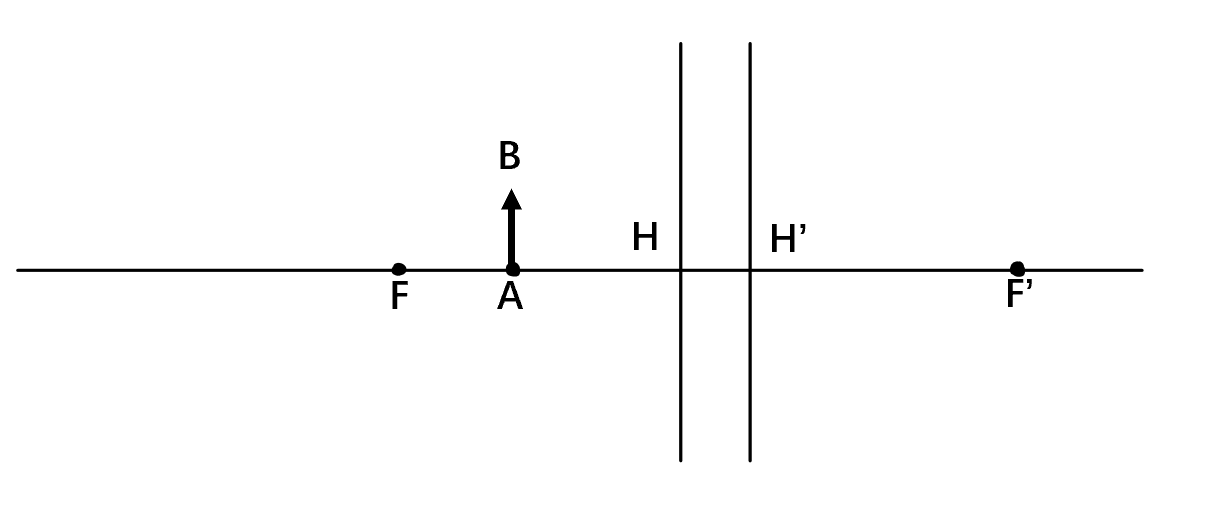
\includegraphics[scale=0.2]{3.png}% 插入图片,按50%的比例缩放
    \end{itemize}
    \subsection*{3.(新题)照相物镜焦距为$50mm$,相对空间1:5,对$2m$远处照相,假定底片上弥散斑直径小于$0.05mm$时,仍可以认为成像清晰,问物空间能清晰成像的最远、最近距离是多少?}
    \vspace{20mm}
    \subsection*{4.(13年6题)今有一振动方向与入射面的法线成$45\degree$角的线偏振光以$48\degree37^{'}$角入射到玻璃-空气界面上,玻璃折射率为$n=1.51$。试确定反射光的偏振状态(光电场矢量末端轨迹、旋向),并表示出反射光的归一化琼斯矢量。}
    \vspace{20mm}
    \subsection*{5.(08年第8题,第一问变动)图示方解石棱镜的主折射率为$n_o=1.6408$,$n_e=1.4790$}
    \begin{itemize}
        \item (1)若要使其称为格兰-傅科棱镜工作,说明格兰-傅科棱镜的作用原理。
        \vspace{-3mm}
        \item (2)当如图斜入射-平行光,入射角$\phi $为多大时该格兰-傅科棱镜工作失效。
        \vspace{-3mm}
    \end{itemize}
    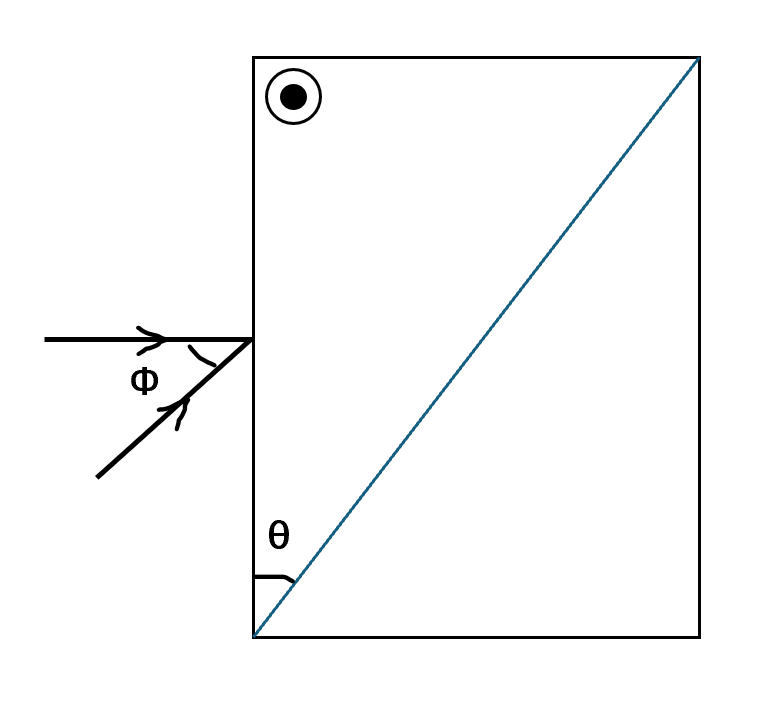
\includegraphics[scale=0.3]{4.png}
    \vspace{20mm}
    \subsection*{6.(08年第13题)我国发射了月球探测卫星,已知月球半径$R=1738km$,太阳的辐强度为$I=3X10^{25}\frac{W}{sr}$,太阳到月球的平均距离$l=1.5x10^11m$,求月球接收的辐通量和辐照度。(今年在月球的基础上给了火星的半径和距离,分别求两个的..)}
    %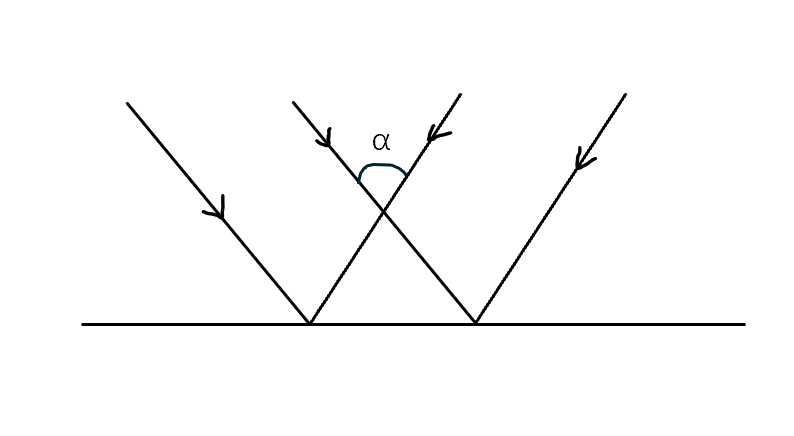
\includegraphics[scale=0.3]{6.png}
    \vspace{20mm}
    \subsection*{7.(08年第14题)$7^{x}$开普勒望远系统,视场$2\omega =8\degree$,目镜焦距为$25mm$,出瞳直径为$5mm$,假定孔径光阑与物镜框重合,系统无渐晕,求:}
    \begin{itemize}
        \vspace{-3mm}
        \item (1)物镜焦距$f_{物}^{'}$;
        \vspace{-3mm}
        \item (2)物镜口径;
        \vspace{-3mm}
        \item (3)分化板直径;
        \vspace{-3mm}
        \item (4)目镜口径。
    \end{itemize}
    \subsection*{8.(10年第1题)如图所示,两相干平面光波其一在xz平面沿与z轴夹角$\theta_1$方向传播,其二在xz平面沿z轴反向传播。试求该两个光波在$z=0$平面上干涉条纹的形状和间距。}
    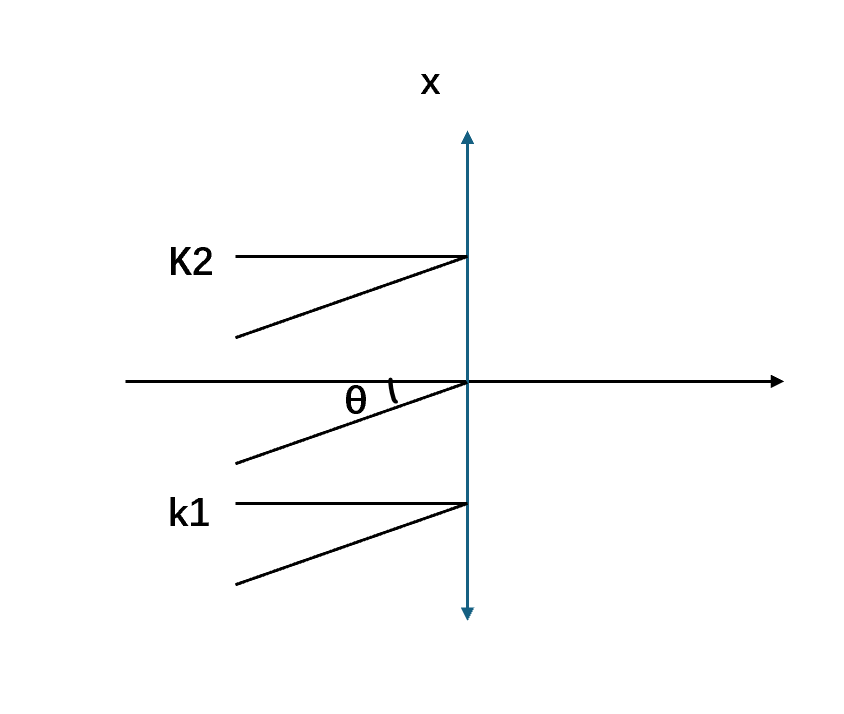
\includegraphics[scale=0.2]{5.png}
    \vspace{15mm}
    \subsection*{9.(10年第6题)在两个正交偏振器之间插入一块$\frac{1}{4}$波片,强度为$I_0$的单色光通过这一系统。如果将波片绕光的传播方向旋转一周,问:}
    \begin{itemize}
        \vspace{-3mm}
        \item (1)将看到几个光强的极大和极小值?计算相应的波片方位及光强数值。
        \vspace{-3mm}
        \item (2)用全波片代替$\frac{1}{4}$波片,情况如何?
    \end{itemize}
    \vspace{15mm}
    \subsection*{10.(16年第8题)今在平板玻璃片上镀一层银膜,然后再在银膜上加镀一层透明介质层,在其上再镀一层银膜,制成一块干涉滤光片。设银膜的反射率为$0.95$;透明介质膜的折射率为1.56;膜后为4$\mu m$。若用一束平行光垂直照射该干涉滤光片,求在$380.0~760.0nm$可见光范围内,透射最强的光谱线数目,相应的波长和谱线的线宽。}
    \vspace{15mm}
    \subsection*{11.(新题)平行白光照射$d=1mm$双缝,用焦距1m的透镜将衍射光聚焦在观察屏上,若在屏上距中央白纹$3mm$处观测,可见光区缺哪些波长?屏上观测到可见光两边缘波长的二级极大之间距离。}
    \vspace{15mm}
    \subsection*{12.(10年第13题)有一架开普勒望远镜,视放大率$\Gamma $为6,物方视场角$2\omega =8\degree$,出瞳直径为$D^{'}=5mm$,物镜和目镜之间的距离$L=140mm$,假定孔径光阑与物镜框重合,系统无渐晕,求:}
    \begin{itemize}
        \vspace{-3mm}
        \item (1) 物镜焦距$f_{物}^{'}$和目镜焦距$f_{目}^{'}$;
        \vspace{-3mm}
        \item (2)
        \vspace{-3mm}
        \item (3)
    \end{itemize}
    %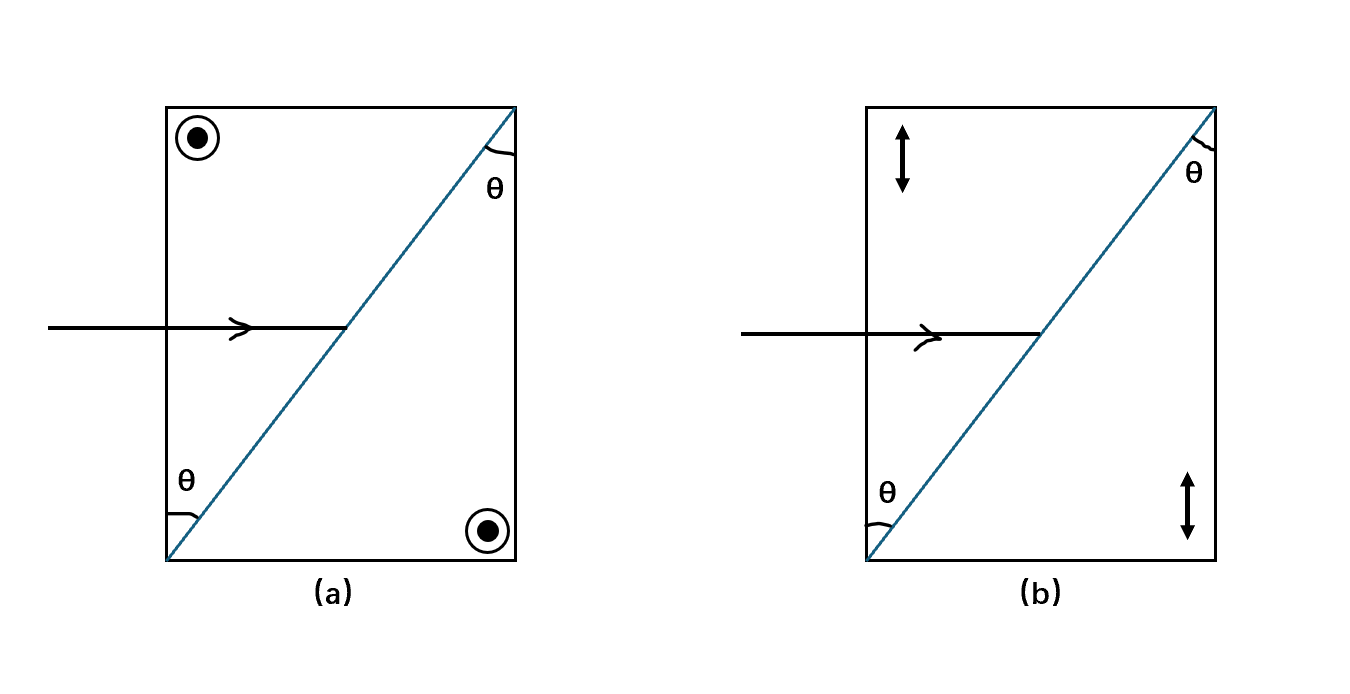
\includegraphics[scale=0.3]{7.png}
\end{document}